\documentclass[1p]{elsarticle_modified}
%\bibliographystyle{elsarticle-num}

%\usepackage[colorlinks]{hyperref}
%\usepackage{abbrmath_seonhwa} %\Abb, \Ascr, \Acal ,\Abf, \Afrak
\usepackage{amsfonts}
\usepackage{amssymb}
\usepackage{amsmath}
\usepackage{amsthm}
\usepackage{scalefnt}
\usepackage{amsbsy}
\usepackage{kotex}
\usepackage{caption}
\usepackage{subfig}
\usepackage{color}
\usepackage{graphicx}
\usepackage{xcolor} %% white, black, red, green, blue, cyan, magenta, yellow
\usepackage{float}
\usepackage{setspace}
\usepackage{hyperref}

\usepackage{tikz}
\usetikzlibrary{arrows}

\usepackage{multirow}
\usepackage{array} % fixed length table
\usepackage{hhline}

%%%%%%%%%%%%%%%%%%%%%
\makeatletter
\renewcommand*\env@matrix[1][\arraystretch]{%
	\edef\arraystretch{#1}%
	\hskip -\arraycolsep
	\let\@ifnextchar\new@ifnextchar
	\array{*\c@MaxMatrixCols c}}
\makeatother %https://tex.stackexchange.com/questions/14071/how-can-i-increase-the-line-spacing-in-a-matrix
%%%%%%%%%%%%%%%

\usepackage[normalem]{ulem}

\newcommand{\msout}[1]{\ifmmode\text{\sout{\ensuremath{#1}}}\else\sout{#1}\fi}
%SOURCE: \msout is \stkout macro in https://tex.stackexchange.com/questions/20609/strikeout-in-math-mode

\newcommand{\cancel}[1]{
	\ifmmode
	{\color{red}\msout{#1}}
	\else
	{\color{red}\sout{#1}}
	\fi
}

\newcommand{\add}[1]{
	{\color{blue}\uwave{#1}}
}

\newcommand{\replace}[2]{
	\ifmmode
	{\color{red}\msout{#1}}{\color{blue}\uwave{#2}}
	\else
	{\color{red}\sout{#1}}{\color{blue}\uwave{#2}}
	\fi
}

\newcommand{\Sol}{\mathcal{S}} %segment
\newcommand{\D}{D} %diagram
\newcommand{\A}{\mathcal{A}} %arc


%%%%%%%%%%%%%%%%%%%%%%%%%%%%%5 test

\def\sl{\operatorname{\textup{SL}}(2,\Cbb)}
\def\psl{\operatorname{\textup{PSL}}(2,\Cbb)}
\def\quan{\mkern 1mu \triangleright \mkern 1mu}

\theoremstyle{definition}
\newtheorem{thm}{Theorem}[section]
\newtheorem{prop}[thm]{Proposition}
\newtheorem{lem}[thm]{Lemma}
\newtheorem{ques}[thm]{Question}
\newtheorem{cor}[thm]{Corollary}
\newtheorem{defn}[thm]{Definition}
\newtheorem{exam}[thm]{Example}
\newtheorem{rmk}[thm]{Remark}
\newtheorem{alg}[thm]{Algorithm}

\newcommand{\I}{\sqrt{-1}}
\begin{document}

%\begin{frontmatter}
%
%\title{Boundary parabolic representations of knots up to 8 crossings}
%
%%% Group authors per affiliation:
%\author{Yunhi Cho} 
%\address{Department of Mathematics, University of Seoul, Seoul, Korea}
%\ead{yhcho@uos.ac.kr}
%
%
%\author{Seonhwa Kim} %\fnref{s_kim}}
%\address{Center for Geometry and Physics, Institute for Basic Science, Pohang, 37673, Korea}
%\ead{ryeona17@ibs.re.kr}
%
%\author{Hyuk Kim}
%\address{Department of Mathematical Sciences, Seoul National University, Seoul 08826, Korea}
%\ead{hyukkim@snu.ac.kr}
%
%\author{Seokbeom Yoon}
%\address{Department of Mathematical Sciences, Seoul National University, Seoul, 08826,  Korea}
%\ead{sbyoon15@snu.ac.kr}
%
%\begin{abstract}
%We find all boundary parabolic representation of knots up to 8 crossings.
%
%\end{abstract}
%\begin{keyword}
%    \MSC[2010] 57M25 
%\end{keyword}
%
%\end{frontmatter}

%\linenumbers
%\tableofcontents
%
\newcommand\colored[1]{\textcolor{white}{\rule[-0.35ex]{0.8em}{1.4ex}}\kern-0.8em\color{red} #1}%
%\newcommand\colored[1]{\textcolor{white}{ #1}\kern-2.17ex	\textcolor{white}{ #1}\kern-1.81ex	\textcolor{white}{ #1}\kern-2.15ex\color{red}#1	}

{\Large $\underline{11a_{112}~(K11a_{112})}$}

\setlength{\tabcolsep}{10pt}
\renewcommand{\arraystretch}{1.6}
\vspace{1cm}\begin{tabular}{m{100pt}>{\centering\arraybackslash}m{274pt}}
\multirow{5}{120pt}{
	\centering
	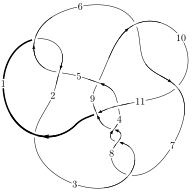
\includegraphics[width=112pt]{../../../GIT/diagram.site/Diagrams/png/361_11a_112.png}\\
\ \ \ A knot diagram\footnotemark}&
\allowdisplaybreaks
\textbf{Linearized knot diagam} \\
\cline{2-2}
 &
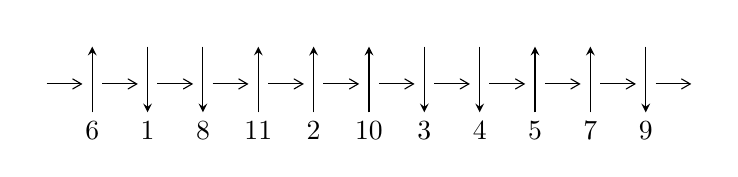
\begin{tikzpicture}[x=20pt, y=17pt]
	% nodes
	\node (C0) at (0, 0) {};
	\node (C1) at (1, 0) {};
	\node (C1U) at (1, +1) {};
	\node (C1D) at (1, -1) {6};

	\node (C2) at (2, 0) {};
	\node (C2U) at (2, +1) {};
	\node (C2D) at (2, -1) {1};

	\node (C3) at (3, 0) {};
	\node (C3U) at (3, +1) {};
	\node (C3D) at (3, -1) {8};

	\node (C4) at (4, 0) {};
	\node (C4U) at (4, +1) {};
	\node (C4D) at (4, -1) {11};

	\node (C5) at (5, 0) {};
	\node (C5U) at (5, +1) {};
	\node (C5D) at (5, -1) {2};

	\node (C6) at (6, 0) {};
	\node (C6U) at (6, +1) {};
	\node (C6D) at (6, -1) {10};

	\node (C7) at (7, 0) {};
	\node (C7U) at (7, +1) {};
	\node (C7D) at (7, -1) {3};

	\node (C8) at (8, 0) {};
	\node (C8U) at (8, +1) {};
	\node (C8D) at (8, -1) {4};

	\node (C9) at (9, 0) {};
	\node (C9U) at (9, +1) {};
	\node (C9D) at (9, -1) {5};

	\node (C10) at (10, 0) {};
	\node (C10U) at (10, +1) {};
	\node (C10D) at (10, -1) {7};

	\node (C11) at (11, 0) {};
	\node (C11U) at (11, +1) {};
	\node (C11D) at (11, -1) {9};
	\node (C12) at (12, 0) {};

	% arrows
	\draw[->,>={angle 60}]
	(C0) edge (C1) (C1) edge (C2) (C2) edge (C3) (C3) edge (C4) (C4) edge (C5) (C5) edge (C6) (C6) edge (C7) (C7) edge (C8) (C8) edge (C9) (C9) edge (C10) (C10) edge (C11) (C11) edge (C12) ;	\draw[->,>=stealth]
	(C1D) edge (C1U) (C2U) edge (C2D) (C3U) edge (C3D) (C4D) edge (C4U) (C5D) edge (C5U) (C6D) edge (C6U) (C7U) edge (C7D) (C8U) edge (C8D) (C9D) edge (C9U) (C10D) edge (C10U) (C11U) edge (C11D) ;
	\end{tikzpicture} \\
\hhline{~~} \\& 
\textbf{Solving Sequence} \\ \cline{2-2} 
 &
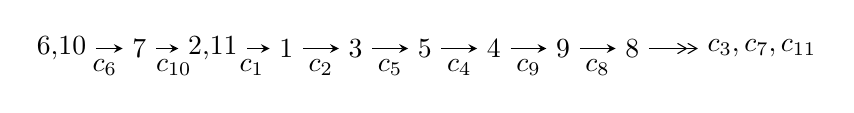
\begin{tikzpicture}[x=25pt, y=7pt]
	% node
	\node (A0) at (-1/8, 0) {6,10};
	\node (A1) at (1, 0) {7};
	\node (A2) at (33/16, 0) {2,11};
	\node (A3) at (25/8, 0) {1};
	\node (A4) at (33/8, 0) {3};
	\node (A5) at (41/8, 0) {5};
	\node (A6) at (49/8, 0) {4};
	\node (A7) at (57/8, 0) {9};
	\node (A8) at (65/8, 0) {8};
	\node (C1) at (1/2, -1) {$c_{6}$};
	\node (C2) at (3/2, -1) {$c_{10}$};
	\node (C3) at (21/8, -1) {$c_{1}$};
	\node (C4) at (29/8, -1) {$c_{2}$};
	\node (C5) at (37/8, -1) {$c_{5}$};
	\node (C6) at (45/8, -1) {$c_{4}$};
	\node (C7) at (53/8, -1) {$c_{9}$};
	\node (C8) at (61/8, -1) {$c_{8}$};
	\node (A9) at (10, 0) {$c_{3},c_{7},c_{11}$};

	% edge
	\draw[->,>=stealth]	
	(A0) edge (A1) (A1) edge (A2) (A2) edge (A3) (A3) edge (A4) (A4) edge (A5) (A5) edge (A6) (A6) edge (A7) (A7) edge (A8) ;
	\draw[->>,>={angle 60}]	
	(A8) edge (A9);
\end{tikzpicture} \\ 

\end{tabular} \\

\footnotetext{
The image of knot diagram is generated by the software ``\textbf{Draw programme}" developed by Andrew Bartholomew(\url{http://www.layer8.co.uk/maths/draw/index.htm\#Running-draw}), where we modified some parts for our purpose(\url{https://github.com/CATsTAILs/LinksPainter}).
}\phantom \\ \newline 
\centering \textbf{Ideals for irreducible components\footnotemark of $X_{\text{par}}$} 
 
\begin{align*}
I^u_{1}&=\langle 
-8.66742\times10^{142} u^{65}-1.85341\times10^{143} u^{64}+\cdots+5.23974\times10^{142} b-3.98318\times10^{145},\\
\phantom{I^u_{1}}&\phantom{= \langle  }-2.38832\times10^{145} u^{65}-5.07173\times10^{145} u^{64}+\cdots+2.04874\times10^{145} a-1.06078\times10^{148},\\
\phantom{I^u_{1}}&\phantom{= \langle  }u^{66}+3 u^{65}+\cdots-698 u+391\rangle \\
I^u_{2}&=\langle 
u^{12}-2 u^{11}-5 u^{10}+12 u^9+8 u^8-29 u^7+34 u^5-13 u^4-18 u^3+13 u^2+b+3 u-3,\\
\phantom{I^u_{2}}&\phantom{= \langle  }- u^{13}+4 u^{12}+u^{11}-22 u^{10}+16 u^9+45 u^8-58 u^7-35 u^6+83 u^5-6 u^4-54 u^3+23 u^2+a+11 u-7,\\
\phantom{I^u_{2}}&\phantom{= \langle  }u^{14}-2 u^{13}-5 u^{12}+12 u^{11}+8 u^{10}-29 u^9+35 u^7-14 u^6-21 u^5+16 u^4+5 u^3-6 u^2+1\rangle \\
I^u_{3}&=\langle 
- u^5+2 u^4+u^3-2 u^2+b- u,\;- u^5+2 u^4+2 u^3-4 u^2+a- u,\\
\phantom{I^u_{3}}&\phantom{= \langle  }u^{10}-4 u^9+2 u^8+8 u^7-5 u^6-7 u^5+3 u^3+3 u^2+u+1\rangle \\
\\
\end{align*}
\raggedright * 3 irreducible components of $\dim_{\mathbb{C}}=0$, with total 90 representations.\\
\footnotetext{All coefficients of polynomials are rational numbers. But the coefficients are sometimes approximated in decimal forms when there is not enough margin.}
\newpage
\renewcommand{\arraystretch}{1}
\centering \section*{I. $I^u_{1}= \langle -8.67\times10^{142} u^{65}-1.85\times10^{143} u^{64}+\cdots+5.24\times10^{142} b-3.98\times10^{145},\;-2.39\times10^{145} u^{65}-5.07\times10^{145} u^{64}+\cdots+2.05\times10^{145} a-1.06\times10^{148},\;u^{66}+3 u^{65}+\cdots-698 u+391 \rangle$}
\flushleft \textbf{(i) Arc colorings}\\
\begin{tabular}{m{7pt} m{180pt} m{7pt} m{180pt} }
\flushright $a_{6}=$&$\begin{pmatrix}1\\0\end{pmatrix}$ \\
\flushright $a_{10}=$&$\begin{pmatrix}0\\u\end{pmatrix}$ \\
\flushright $a_{7}=$&$\begin{pmatrix}1\\- u^2\end{pmatrix}$ \\
\flushright $a_{2}=$&$\begin{pmatrix}1.16575 u^{65}+2.47554 u^{64}+\cdots-1496.97 u+517.772\\1.65417 u^{65}+3.53723 u^{64}+\cdots-2227.88 u+760.187\end{pmatrix}$ \\
\flushright $a_{11}=$&$\begin{pmatrix}u\\- u^3+u\end{pmatrix}$ \\
\flushright $a_{1}=$&$\begin{pmatrix}-0.488417 u^{65}-1.06169 u^{64}+\cdots+730.907 u-242.415\\1.65417 u^{65}+3.53723 u^{64}+\cdots-2227.88 u+760.187\end{pmatrix}$ \\
\flushright $a_{3}=$&$\begin{pmatrix}-4.63396 u^{65}-9.87610 u^{64}+\cdots+6180.95 u-2106.10\\3.44579 u^{65}+7.31099 u^{64}+\cdots-4516.19 u+1545.50\end{pmatrix}$ \\
\flushright $a_{5}=$&$\begin{pmatrix}-1.21103 u^{65}-2.58621 u^{64}+\cdots+1614.03 u-550.273\\2.65367 u^{65}+5.65967 u^{64}+\cdots-3544.37 u+1207.93\end{pmatrix}$ \\
\flushright $a_{4}=$&$\begin{pmatrix}-3.44270 u^{65}-7.34774 u^{64}+\cdots+4580.96 u-1560.01\\2.08906 u^{65}+4.45851 u^{64}+\cdots-2799.61 u+954.194\end{pmatrix}$ \\
\flushright $a_{9}=$&$\begin{pmatrix}1.82812 u^{65}+3.88511 u^{64}+\cdots-2437.77 u+836.494\\-1.49101 u^{65}-3.16113 u^{64}+\cdots+1941.13 u-660.317\end{pmatrix}$ \\
\flushright $a_{8}=$&$\begin{pmatrix}6.19671 u^{65}+13.2052 u^{64}+\cdots-8254.78 u+2813.85\\-4.20938 u^{65}-8.93733 u^{64}+\cdots+5543.38 u-1893.47\end{pmatrix}$\\ \flushright $a_{8}=$&$\begin{pmatrix}6.19671 u^{65}+13.2052 u^{64}+\cdots-8254.78 u+2813.85\\-4.20938 u^{65}-8.93733 u^{64}+\cdots+5543.38 u-1893.47\end{pmatrix}$\\&\end{tabular}
\flushleft \textbf{(ii) Obstruction class $= -1$}\\~\\
\flushleft \textbf{(iii) Cusp Shapes $= -4.78436 u^{65}-10.2758 u^{64}+\cdots+6384.50 u-2162.36$}\\~\\
\newpage\renewcommand{\arraystretch}{1}
\flushleft \textbf{(iv) u-Polynomials at the component}\newline \\
\begin{tabular}{m{50pt}|m{274pt}}
Crossings & \hspace{64pt}u-Polynomials at each crossing \\
\hline $$\begin{aligned}c_{1},c_{5}\end{aligned}$$&$\begin{aligned}
&u^{66}+5 u^{65}+\cdots+34 u+4
\end{aligned}$\\
\hline $$\begin{aligned}c_{2}\end{aligned}$$&$\begin{aligned}
&u^{66}+27 u^{65}+\cdots-12 u+16
\end{aligned}$\\
\hline $$\begin{aligned}c_{3},c_{7},c_{8}\end{aligned}$$&$\begin{aligned}
&u^{66}- u^{65}+\cdots-56 u+11
\end{aligned}$\\
\hline $$\begin{aligned}c_{4}\end{aligned}$$&$\begin{aligned}
&u^{66}-3 u^{65}+\cdots-250 u+71
\end{aligned}$\\
\hline $$\begin{aligned}c_{6},c_{10}\end{aligned}$$&$\begin{aligned}
&u^{66}-3 u^{65}+\cdots+698 u+391
\end{aligned}$\\
\hline $$\begin{aligned}c_{9}\end{aligned}$$&$\begin{aligned}
&u^{66}+u^{65}+\cdots-470 u+241
\end{aligned}$\\
\hline $$\begin{aligned}c_{11}\end{aligned}$$&$\begin{aligned}
&u^{66}-7 u^{65}+\cdots-102 u-67
\end{aligned}$\\
\hline
\end{tabular}\\~\\
\newpage\renewcommand{\arraystretch}{1}
\flushleft \textbf{(v) Riley Polynomials at the component}\newline \\
\begin{tabular}{m{50pt}|m{274pt}}
Crossings & \hspace{64pt}Riley Polynomials at each crossing \\
\hline $$\begin{aligned}c_{1},c_{5}\end{aligned}$$&$\begin{aligned}
&y^{66}+27 y^{65}+\cdots-12 y+16
\end{aligned}$\\
\hline $$\begin{aligned}c_{2}\end{aligned}$$&$\begin{aligned}
&y^{66}+27 y^{65}+\cdots-164976 y+256
\end{aligned}$\\
\hline $$\begin{aligned}c_{3},c_{7},c_{8}\end{aligned}$$&$\begin{aligned}
&y^{66}-69 y^{65}+\cdots+3574 y+121
\end{aligned}$\\
\hline $$\begin{aligned}c_{4}\end{aligned}$$&$\begin{aligned}
&y^{66}+13 y^{65}+\cdots+99380 y+5041
\end{aligned}$\\
\hline $$\begin{aligned}c_{6},c_{10}\end{aligned}$$&$\begin{aligned}
&y^{66}-41 y^{65}+\cdots-3193706 y+152881
\end{aligned}$\\
\hline $$\begin{aligned}c_{9}\end{aligned}$$&$\begin{aligned}
&y^{66}-21 y^{65}+\cdots-54610 y+58081
\end{aligned}$\\
\hline $$\begin{aligned}c_{11}\end{aligned}$$&$\begin{aligned}
&y^{66}-3 y^{65}+\cdots-228020 y+4489
\end{aligned}$\\
\hline
\end{tabular}\\~\\
\newpage\flushleft \textbf{(vi) Complex Volumes and Cusp Shapes}
$$\begin{array}{c|c|c}  
\text{Solutions to }I^u_{1}& \I (\text{vol} + \sqrt{-1}CS) & \text{Cusp shape}\\
 \hline 
\begin{aligned}
u &= \phantom{-}0.553994 + 0.817132 I \\
a &= \phantom{-}0.58544 + 1.58860 I \\
b &= \phantom{-}0.070442 + 0.432736 I\end{aligned}
 & -4.89628 + 4.04600 I & \phantom{-0.000000 } 0. - 7.91470 I \\ \hline\begin{aligned}
u &= \phantom{-}0.553994 - 0.817132 I \\
a &= \phantom{-}0.58544 - 1.58860 I \\
b &= \phantom{-}0.070442 - 0.432736 I\end{aligned}
 & -4.89628 - 4.04600 I & \phantom{-0.000000 -}0. + 7.91470 I \\ \hline\begin{aligned}
u &= \phantom{-}0.044651 + 1.027560 I \\
a &= -0.03585 - 1.60708 I \\
b &= \phantom{-}0.595192 - 0.987582 I\end{aligned}
 & -0.53608 - 6.26556 I & \phantom{-0.000000 -}0. + 8.67399 I \\ \hline\begin{aligned}
u &= \phantom{-}0.044651 - 1.027560 I \\
a &= -0.03585 + 1.60708 I \\
b &= \phantom{-}0.595192 + 0.987582 I\end{aligned}
 & -0.53608 + 6.26556 I & \phantom{-0.000000 } 0. - 8.67399 I \\ \hline\begin{aligned}
u &= -1.057280 + 0.123271 I \\
a &= -0.299700 + 0.067824 I \\
b &= \phantom{-}1.073380 - 0.701395 I\end{aligned}
 & \phantom{-}0.04052 - 3.80627 I & \phantom{-0.000000 } 0 \\ \hline\begin{aligned}
u &= -1.057280 - 0.123271 I \\
a &= -0.299700 - 0.067824 I \\
b &= \phantom{-}1.073380 + 0.701395 I\end{aligned}
 & \phantom{-}0.04052 + 3.80627 I & \phantom{-0.000000 } 0 \\ \hline\begin{aligned}
u &= \phantom{-}0.580719 + 0.732261 I \\
a &= -0.07117 + 1.86879 I \\
b &= \phantom{-}0.428988 + 1.124710 I\end{aligned}
 & -7.34513 + 3.69328 I & -5.70329 - 3.99766 I \\ \hline\begin{aligned}
u &= \phantom{-}0.580719 - 0.732261 I \\
a &= -0.07117 - 1.86879 I \\
b &= \phantom{-}0.428988 - 1.124710 I\end{aligned}
 & -7.34513 - 3.69328 I & -5.70329 + 3.99766 I \\ \hline\begin{aligned}
u &= -0.546154 + 0.917664 I \\
a &= \phantom{-}1.02255 + 1.19790 I \\
b &= -0.178208 + 1.154380 I\end{aligned}
 & -9.63085 + 2.05112 I & \phantom{-0.000000 } 0 \\ \hline\begin{aligned}
u &= -0.546154 - 0.917664 I \\
a &= \phantom{-}1.02255 - 1.19790 I \\
b &= -0.178208 - 1.154380 I\end{aligned}
 & -9.63085 - 2.05112 I & \phantom{-0.000000 } 0\\
 \hline 
 \end{array}$$\newpage$$\begin{array}{c|c|c}  
\text{Solutions to }I^u_{1}& \I (\text{vol} + \sqrt{-1}CS) & \text{Cusp shape}\\
 \hline 
\begin{aligned}
u &= \phantom{-}1.024070 + 0.311697 I \\
a &= \phantom{-}0.41730 - 1.46428 I \\
b &= -0.032613 - 1.192350 I\end{aligned}
 & -1.28697 + 4.18216 I & \phantom{-0.000000 } 0 \\ \hline\begin{aligned}
u &= \phantom{-}1.024070 - 0.311697 I \\
a &= \phantom{-}0.41730 + 1.46428 I \\
b &= -0.032613 + 1.192350 I\end{aligned}
 & -1.28697 - 4.18216 I & \phantom{-0.000000 } 0 \\ \hline\begin{aligned}
u &= -0.197995 + 0.874170 I \\
a &= \phantom{-}0.140181 + 0.842371 I \\
b &= \phantom{-}0.574376 + 0.595359 I\end{aligned}
 & \phantom{-}0.60022 - 1.53805 I & \phantom{-}2.72682 + 4.17703 I \\ \hline\begin{aligned}
u &= -0.197995 - 0.874170 I \\
a &= \phantom{-}0.140181 - 0.842371 I \\
b &= \phantom{-}0.574376 - 0.595359 I\end{aligned}
 & \phantom{-}0.60022 + 1.53805 I & \phantom{-}2.72682 - 4.17703 I \\ \hline\begin{aligned}
u &= \phantom{-}0.057515 + 1.110030 I \\
a &= \phantom{-}0.176652 + 0.885390 I \\
b &= -0.641007 + 0.405819 I\end{aligned}
 & -5.13042 + 4.43339 I & \phantom{-0.000000 } 0 \\ \hline\begin{aligned}
u &= \phantom{-}0.057515 - 1.110030 I \\
a &= \phantom{-}0.176652 - 0.885390 I \\
b &= -0.641007 - 0.405819 I\end{aligned}
 & -5.13042 - 4.43339 I & \phantom{-0.000000 } 0 \\ \hline\begin{aligned}
u &= -0.866529 + 0.013355 I \\
a &= -1.33674 + 0.64592 I \\
b &= \phantom{-}0.873691 + 1.006930 I\end{aligned}
 & -0.89589 + 3.10402 I & \phantom{-}0.54343 - 3.05170 I \\ \hline\begin{aligned}
u &= -0.866529 - 0.013355 I \\
a &= -1.33674 - 0.64592 I \\
b &= \phantom{-}0.873691 - 1.006930 I\end{aligned}
 & -0.89589 - 3.10402 I & \phantom{-}0.54343 + 3.05170 I \\ \hline\begin{aligned}
u &= \phantom{-}0.853665 + 0.135106 I \\
a &= -2.43454 + 0.28897 I \\
b &= \phantom{-}0.505356 - 0.698814 I\end{aligned}
 & -4.10664 + 2.85933 I & \phantom{-}0.363943 - 0.476166 I \\ \hline\begin{aligned}
u &= \phantom{-}0.853665 - 0.135106 I \\
a &= -2.43454 - 0.28897 I \\
b &= \phantom{-}0.505356 + 0.698814 I\end{aligned}
 & -4.10664 - 2.85933 I & \phantom{-}0.363943 + 0.476166 I\\
 \hline 
 \end{array}$$\newpage$$\begin{array}{c|c|c}  
\text{Solutions to }I^u_{1}& \I (\text{vol} + \sqrt{-1}CS) & \text{Cusp shape}\\
 \hline 
\begin{aligned}
u &= -1.032450 + 0.507113 I \\
a &= -0.217969 - 1.258850 I \\
b &= \phantom{-}0.038438 - 1.392570 I\end{aligned}
 & -8.05212 - 7.21112 I & \phantom{-0.000000 } 0 \\ \hline\begin{aligned}
u &= -1.032450 - 0.507113 I \\
a &= -0.217969 + 1.258850 I \\
b &= \phantom{-}0.038438 + 1.392570 I\end{aligned}
 & -8.05212 + 7.21112 I & \phantom{-0.000000 } 0 \\ \hline\begin{aligned}
u &= \phantom{-}1.144210 + 0.214797 I \\
a &= \phantom{-}0.961366 - 0.866826 I \\
b &= -0.744120 - 1.117900 I\end{aligned}
 & \phantom{-}2.95387 + 4.62224 I & \phantom{-0.000000 } 0 \\ \hline\begin{aligned}
u &= \phantom{-}1.144210 - 0.214797 I \\
a &= \phantom{-}0.961366 + 0.866826 I \\
b &= -0.744120 + 1.117900 I\end{aligned}
 & \phantom{-}2.95387 - 4.62224 I & \phantom{-0.000000 } 0 \\ \hline\begin{aligned}
u &= \phantom{-}1.136700 + 0.303584 I \\
a &= -1.56569 - 0.14302 I \\
b &= \phantom{-}0.543699 + 0.963909 I\end{aligned}
 & -4.97139 + 7.17182 I & \phantom{-0.000000 } 0 \\ \hline\begin{aligned}
u &= \phantom{-}1.136700 - 0.303584 I \\
a &= -1.56569 + 0.14302 I \\
b &= \phantom{-}0.543699 - 0.963909 I\end{aligned}
 & -4.97139 - 7.17182 I & \phantom{-0.000000 } 0 \\ \hline\begin{aligned}
u &= -0.809325 + 0.115865 I \\
a &= -0.52327 - 2.10152 I \\
b &= -0.215765 - 1.035700 I\end{aligned}
 & -0.545532 + 0.599797 I & \phantom{-}1.64339 + 2.56314 I \\ \hline\begin{aligned}
u &= -0.809325 - 0.115865 I \\
a &= -0.52327 + 2.10152 I \\
b &= -0.215765 + 1.035700 I\end{aligned}
 & -0.545532 - 0.599797 I & \phantom{-}1.64339 - 2.56314 I \\ \hline\begin{aligned}
u &= -1.118470 + 0.456780 I \\
a &= \phantom{-}1.17750 + 1.75389 I \\
b &= -0.605458 + 1.064560 I\end{aligned}
 & \phantom{-}2.13300 - 6.10455 I & \phantom{-0.000000 } 0 \\ \hline\begin{aligned}
u &= -1.118470 - 0.456780 I \\
a &= \phantom{-}1.17750 - 1.75389 I \\
b &= -0.605458 - 1.064560 I\end{aligned}
 & \phantom{-}2.13300 + 6.10455 I & \phantom{-0.000000 } 0\\
 \hline 
 \end{array}$$\newpage$$\begin{array}{c|c|c}  
\text{Solutions to }I^u_{1}& \I (\text{vol} + \sqrt{-1}CS) & \text{Cusp shape}\\
 \hline 
\begin{aligned}
u &= \phantom{-}1.209870 + 0.001472 I \\
a &= \phantom{-}0.291036 - 0.003235 I \\
b &= -0.958064 - 0.487956 I\end{aligned}
 & \phantom{-}4.84160 + 1.58290 I & \phantom{-0.000000 } 0 \\ \hline\begin{aligned}
u &= \phantom{-}1.209870 - 0.001472 I \\
a &= \phantom{-}0.291036 + 0.003235 I \\
b &= -0.958064 + 0.487956 I\end{aligned}
 & \phantom{-}4.84160 - 1.58290 I & \phantom{-0.000000 } 0 \\ \hline\begin{aligned}
u &= \phantom{-}0.992580 + 0.743807 I \\
a &= \phantom{-}0.829585 - 0.896312 I \\
b &= \phantom{-}0.333033 - 0.931189 I\end{aligned}
 & -6.28712 + 1.90390 I & \phantom{-0.000000 } 0 \\ \hline\begin{aligned}
u &= \phantom{-}0.992580 - 0.743807 I \\
a &= \phantom{-}0.829585 + 0.896312 I \\
b &= \phantom{-}0.333033 + 0.931189 I\end{aligned}
 & -6.28712 - 1.90390 I & \phantom{-0.000000 } 0 \\ \hline\begin{aligned}
u &= \phantom{-}0.661473 + 0.362026 I \\
a &= \phantom{-}0.388489 - 0.220994 I \\
b &= \phantom{-}0.758076 + 0.048117 I\end{aligned}
 & -3.94345 - 0.27627 I & -0.20377 - 1.42170 I \\ \hline\begin{aligned}
u &= \phantom{-}0.661473 - 0.362026 I \\
a &= \phantom{-}0.388489 + 0.220994 I \\
b &= \phantom{-}0.758076 - 0.048117 I\end{aligned}
 & -3.94345 + 0.27627 I & -0.20377 + 1.42170 I \\ \hline\begin{aligned}
u &= -1.217260 + 0.293215 I \\
a &= -0.209546 + 0.352710 I \\
b &= -0.699865 - 0.501839 I\end{aligned}
 & \phantom{-}3.79937 - 1.04615 I & \phantom{-0.000000 } 0 \\ \hline\begin{aligned}
u &= -1.217260 - 0.293215 I \\
a &= -0.209546 - 0.352710 I \\
b &= -0.699865 + 0.501839 I\end{aligned}
 & \phantom{-}3.79937 + 1.04615 I & \phantom{-0.000000 } 0 \\ \hline\begin{aligned}
u &= \phantom{-}0.289729 + 0.632525 I \\
a &= -1.20205 + 2.02084 I \\
b &= \phantom{-}0.099360 + 0.983650 I\end{aligned}
 & -3.46107 - 0.67912 I & -7.42755 + 0.90755 I \\ \hline\begin{aligned}
u &= \phantom{-}0.289729 - 0.632525 I \\
a &= -1.20205 - 2.02084 I \\
b &= \phantom{-}0.099360 - 0.983650 I\end{aligned}
 & -3.46107 + 0.67912 I & -7.42755 - 0.90755 I\\
 \hline 
 \end{array}$$\newpage$$\begin{array}{c|c|c}  
\text{Solutions to }I^u_{1}& \I (\text{vol} + \sqrt{-1}CS) & \text{Cusp shape}\\
 \hline 
\begin{aligned}
u &= -1.31931\phantom{ +0.000000I} \\
a &= -0.452314\phantom{ +0.000000I} \\
b &= \phantom{-}0.200297\phantom{ +0.000000I}\end{aligned}
 & \phantom{-}2.96244\phantom{ +0.000000I} & \phantom{-0.000000 } 0 \\ \hline\begin{aligned}
u &= -1.33669\phantom{ +0.000000I} \\
a &= -0.327933\phantom{ +0.000000I} \\
b &= \phantom{-}1.10352\phantom{ +0.000000I}\end{aligned}
 & \phantom{-}1.97498\phantom{ +0.000000I} & \phantom{-0.000000 } 0 \\ \hline\begin{aligned}
u &= -1.336450 + 0.216760 I \\
a &= -0.754740 - 0.809320 I \\
b &= \phantom{-}0.69935 - 1.27364 I\end{aligned}
 & -1.61048 - 6.33014 I & \phantom{-0.000000 } 0 \\ \hline\begin{aligned}
u &= -1.336450 - 0.216760 I \\
a &= -0.754740 + 0.809320 I \\
b &= \phantom{-}0.69935 + 1.27364 I\end{aligned}
 & -1.61048 + 6.33014 I & \phantom{-0.000000 } 0 \\ \hline\begin{aligned}
u &= \phantom{-}1.313190 + 0.421616 I \\
a &= -0.007522 + 0.224374 I \\
b &= \phantom{-}0.882628 - 0.511949 I\end{aligned}
 & \phantom{-}5.12672 + 6.11193 I & \phantom{-0.000000 } 0 \\ \hline\begin{aligned}
u &= \phantom{-}1.313190 - 0.421616 I \\
a &= -0.007522 - 0.224374 I \\
b &= \phantom{-}0.882628 + 0.511949 I\end{aligned}
 & \phantom{-}5.12672 - 6.11193 I & \phantom{-0.000000 } 0 \\ \hline\begin{aligned}
u &= -0.138682 + 1.399980 I \\
a &= \phantom{-}0.020109 - 1.269570 I \\
b &= -0.589344 - 1.066960 I\end{aligned}
 & -6.95817 + 9.29076 I & \phantom{-0.000000 } 0 \\ \hline\begin{aligned}
u &= -0.138682 - 1.399980 I \\
a &= \phantom{-}0.020109 + 1.269570 I \\
b &= -0.589344 + 1.066960 I\end{aligned}
 & -6.95817 - 9.29076 I & \phantom{-0.000000 } 0 \\ \hline\begin{aligned}
u &= \phantom{-}1.30750 + 0.54957 I \\
a &= -1.06901 + 1.35517 I \\
b &= \phantom{-}0.673865 + 1.105880 I\end{aligned}
 & \phantom{-}3.31701 + 11.86690 I & \phantom{-0.000000 } 0 \\ \hline\begin{aligned}
u &= \phantom{-}1.30750 - 0.54957 I \\
a &= -1.06901 - 1.35517 I \\
b &= \phantom{-}0.673865 - 1.105880 I\end{aligned}
 & \phantom{-}3.31701 - 11.86690 I & \phantom{-0.000000 } 0\\
 \hline 
 \end{array}$$\newpage$$\begin{array}{c|c|c}  
\text{Solutions to }I^u_{1}& \I (\text{vol} + \sqrt{-1}CS) & \text{Cusp shape}\\
 \hline 
\begin{aligned}
u &= -1.35147 + 0.54191 I \\
a &= \phantom{-}0.063163 + 0.131606 I \\
b &= -0.988314 - 0.489276 I\end{aligned}
 & -0.83745 - 10.20370 I & \phantom{-0.000000 } 0 \\ \hline\begin{aligned}
u &= -1.35147 - 0.54191 I \\
a &= \phantom{-}0.063163 - 0.131606 I \\
b &= -0.988314 + 0.489276 I\end{aligned}
 & -0.83745 + 10.20370 I & \phantom{-0.000000 } 0 \\ \hline\begin{aligned}
u &= -0.368991 + 0.379736 I \\
a &= -0.719106 + 0.942094 I \\
b &= -0.194366 + 0.419596 I\end{aligned}
 & \phantom{-}0.210341 - 1.088940 I & \phantom{-}2.71206 + 6.43281 I \\ \hline\begin{aligned}
u &= -0.368991 - 0.379736 I \\
a &= -0.719106 - 0.942094 I \\
b &= -0.194366 - 0.419596 I\end{aligned}
 & \phantom{-}0.210341 + 1.088940 I & \phantom{-}2.71206 - 6.43281 I \\ \hline\begin{aligned}
u &= -1.36359 + 0.61753 I \\
a &= -0.881623 - 1.082620 I \\
b &= \phantom{-}0.636156 - 0.930272 I\end{aligned}
 & \phantom{-}3.70447 - 4.43878 I & \phantom{-0.000000 } 0 \\ \hline\begin{aligned}
u &= -1.36359 - 0.61753 I \\
a &= -0.881623 + 1.082620 I \\
b &= \phantom{-}0.636156 + 0.930272 I\end{aligned}
 & \phantom{-}3.70447 + 4.43878 I & \phantom{-0.000000 } 0 \\ \hline\begin{aligned}
u &= \phantom{-}1.28331 + 0.78007 I \\
a &= \phantom{-}0.160169 + 0.274884 I \\
b &= -0.762107 + 0.779221 I\end{aligned}
 & \phantom{-}0.022290 + 1.139270 I & \phantom{-0.000000 } 0 \\ \hline\begin{aligned}
u &= \phantom{-}1.28331 - 0.78007 I \\
a &= \phantom{-}0.160169 - 0.274884 I \\
b &= -0.762107 - 0.779221 I\end{aligned}
 & \phantom{-}0.022290 - 1.139270 I & \phantom{-0.000000 } 0 \\ \hline\begin{aligned}
u &= -1.47641 + 0.39183 I \\
a &= -0.248686 + 0.207203 I \\
b &= \phantom{-}0.644167 + 0.746103 I\end{aligned}
 & \phantom{-}4.27222 + 0.57322 I & \phantom{-0.000000 } 0 \\ \hline\begin{aligned}
u &= -1.47641 - 0.39183 I \\
a &= -0.248686 - 0.207203 I \\
b &= \phantom{-}0.644167 - 0.746103 I\end{aligned}
 & \phantom{-}4.27222 - 0.57322 I & \phantom{-0.000000 } 0\\
 \hline 
 \end{array}$$\newpage$$\begin{array}{c|c|c}  
\text{Solutions to }I^u_{1}& \I (\text{vol} + \sqrt{-1}CS) & \text{Cusp shape}\\
 \hline 
\begin{aligned}
u &= \phantom{-}0.411878 + 0.216634 I \\
a &= -0.83054 - 2.42396 I \\
b &= \phantom{-}0.446886 - 1.198200 I\end{aligned}
 & -7.34762 - 4.66083 I & -3.40198 - 1.35385 I \\ \hline\begin{aligned}
u &= \phantom{-}0.411878 - 0.216634 I \\
a &= -0.83054 + 2.42396 I \\
b &= \phantom{-}0.446886 + 1.198200 I\end{aligned}
 & -7.34762 + 4.66083 I & -3.40198 + 1.35385 I \\ \hline\begin{aligned}
u &= -1.40430 + 0.66218 I \\
a &= \phantom{-}0.92865 + 1.22021 I \\
b &= -0.703220 + 1.153400 I\end{aligned}
 & -2.8953 - 16.3430 I & \phantom{-0.000000 } 0 \\ \hline\begin{aligned}
u &= -1.40430 - 0.66218 I \\
a &= \phantom{-}0.92865 - 1.22021 I \\
b &= -0.703220 - 1.153400 I\end{aligned}
 & -2.8953 + 16.3430 I & \phantom{-0.000000 } 0 \\ \hline\begin{aligned}
u &= \phantom{-}1.24829 + 0.96945 I \\
a &= \phantom{-}0.789126 - 1.086330 I \\
b &= -0.716542 - 0.934610 I\end{aligned}
 & -0.45544 + 6.74104 I & \phantom{-0.000000 } 0 \\ \hline\begin{aligned}
u &= \phantom{-}1.24829 - 0.96945 I \\
a &= \phantom{-}0.789126 + 1.086330 I \\
b &= -0.716542 + 0.934610 I\end{aligned}
 & -0.45544 - 6.74104 I & \phantom{-0.000000 } 0\\
 \hline 
 \end{array}$$\newpage\newpage\renewcommand{\arraystretch}{1}
\centering \section*{II. $I^u_{2}= \langle u^{12}-2 u^{11}+\cdots+b-3,\;- u^{13}+4 u^{12}+\cdots+a-7,\;u^{14}-2 u^{13}+\cdots-6 u^2+1 \rangle$}
\flushleft \textbf{(i) Arc colorings}\\
\begin{tabular}{m{7pt} m{180pt} m{7pt} m{180pt} }
\flushright $a_{6}=$&$\begin{pmatrix}1\\0\end{pmatrix}$ \\
\flushright $a_{10}=$&$\begin{pmatrix}0\\u\end{pmatrix}$ \\
\flushright $a_{7}=$&$\begin{pmatrix}1\\- u^2\end{pmatrix}$ \\
\flushright $a_{2}=$&$\begin{pmatrix}u^{13}-4 u^{12}+\cdots-11 u+7\\- u^{12}+2 u^{11}+\cdots-3 u+3\end{pmatrix}$ \\
\flushright $a_{11}=$&$\begin{pmatrix}u\\- u^3+u\end{pmatrix}$ \\
\flushright $a_{1}=$&$\begin{pmatrix}u^{13}-3 u^{12}+\cdots-8 u+4\\- u^{12}+2 u^{11}+\cdots-3 u+3\end{pmatrix}$ \\
\flushright $a_{3}=$&$\begin{pmatrix}u^{13}-4 u^{12}+\cdots-6 u+6\\u^7- u^6-3 u^5+3 u^4+2 u^3-3 u^2+u+1\end{pmatrix}$ \\
\flushright $a_{5}=$&$\begin{pmatrix}4 u^{13}-9 u^{12}+\cdots-9 u+3\\u^{13}-2 u^{12}+\cdots-3 u-1\end{pmatrix}$ \\
\flushright $a_{4}=$&$\begin{pmatrix}5 u^{13}-11 u^{12}+\cdots-11 u+3\\2 u^{13}-4 u^{12}+\cdots-4 u-1\end{pmatrix}$ \\
\flushright $a_{9}=$&$\begin{pmatrix}- u^{13}+3 u^{12}+\cdots+10 u-5\\u^{12}-2 u^{11}+\cdots+4 u-4\end{pmatrix}$ \\
\flushright $a_{8}=$&$\begin{pmatrix}-2 u^{13}+3 u^{12}+\cdots+5 u+1\\u^{12}- u^{11}-6 u^{10}+6 u^9+14 u^8-15 u^7-15 u^6+20 u^5+6 u^4-14 u^3+4 u\end{pmatrix}$\\ \flushright $a_{8}=$&$\begin{pmatrix}-2 u^{13}+3 u^{12}+\cdots+5 u+1\\u^{12}- u^{11}-6 u^{10}+6 u^9+14 u^8-15 u^7-15 u^6+20 u^5+6 u^4-14 u^3+4 u\end{pmatrix}$\\&\end{tabular}
\flushleft \textbf{(ii) Obstruction class $= 1$}\\~\\
\flushleft \textbf{(iii) Cusp Shapes $= -7 u^{13}+11 u^{12}+40 u^{11}-69 u^{10}-84 u^9+177 u^8+62 u^7-230 u^6+27 u^5+152 u^4-64 u^3-43 u^2+19 u$}\\~\\
\newpage\renewcommand{\arraystretch}{1}
\flushleft \textbf{(iv) u-Polynomials at the component}\newline \\
\begin{tabular}{m{50pt}|m{274pt}}
Crossings & \hspace{64pt}u-Polynomials at each crossing \\
\hline $$\begin{aligned}c_{1}\end{aligned}$$&$\begin{aligned}
&u^{14}- u^{13}+\cdots- u+1
\end{aligned}$\\
\hline $$\begin{aligned}c_{2}\end{aligned}$$&$\begin{aligned}
&u^{14}+7 u^{13}+\cdots+7 u+1
\end{aligned}$\\
\hline $$\begin{aligned}c_{3}\end{aligned}$$&$\begin{aligned}
&u^{14}-7 u^{12}+\cdots-6 u^2+1
\end{aligned}$\\
\hline $$\begin{aligned}c_{4}\end{aligned}$$&$\begin{aligned}
&u^{14}+3 u^{11}+2 u^{10}+u^8+3 u^6- u^5- u^4-2 u^3+u^2+1
\end{aligned}$\\
\hline $$\begin{aligned}c_{5}\end{aligned}$$&$\begin{aligned}
&u^{14}+u^{13}+\cdots+u+1
\end{aligned}$\\
\hline $$\begin{aligned}c_{6}\end{aligned}$$&$\begin{aligned}
&u^{14}-2 u^{13}+\cdots-6 u^2+1
\end{aligned}$\\
\hline $$\begin{aligned}c_{7},c_{8}\end{aligned}$$&$\begin{aligned}
&u^{14}-7 u^{12}+\cdots-6 u^2+1
\end{aligned}$\\
\hline $$\begin{aligned}c_{9}\end{aligned}$$&$\begin{aligned}
&u^{14}+u^{12}-2 u^{11}- u^{10}- u^9+3 u^8+u^6+2 u^4+3 u^3+1
\end{aligned}$\\
\hline $$\begin{aligned}c_{10}\end{aligned}$$&$\begin{aligned}
&u^{14}+2 u^{13}+\cdots-6 u^2+1
\end{aligned}$\\
\hline $$\begin{aligned}c_{11}\end{aligned}$$&$\begin{aligned}
&u^{14}-2 u^{12}+3 u^{10}- u^9+u^8+7 u^7+2 u^6-2 u^5+2 u^4+2 u^3+u^2+2 u+1
\end{aligned}$\\
\hline
\end{tabular}\\~\\
\newpage\renewcommand{\arraystretch}{1}
\flushleft \textbf{(v) Riley Polynomials at the component}\newline \\
\begin{tabular}{m{50pt}|m{274pt}}
Crossings & \hspace{64pt}Riley Polynomials at each crossing \\
\hline $$\begin{aligned}c_{1},c_{5}\end{aligned}$$&$\begin{aligned}
&y^{14}+7 y^{13}+\cdots+7 y+1
\end{aligned}$\\
\hline $$\begin{aligned}c_{2}\end{aligned}$$&$\begin{aligned}
&y^{14}+7 y^{13}+\cdots+3 y+1
\end{aligned}$\\
\hline $$\begin{aligned}c_{3},c_{7},c_{8}\end{aligned}$$&$\begin{aligned}
&y^{14}-14 y^{13}+\cdots-12 y+1
\end{aligned}$\\
\hline $$\begin{aligned}c_{4}\end{aligned}$$&$\begin{aligned}
&y^{14}+4 y^{12}+\cdots+2 y+1
\end{aligned}$\\
\hline $$\begin{aligned}c_{6},c_{10}\end{aligned}$$&$\begin{aligned}
&y^{14}-14 y^{13}+\cdots-12 y+1
\end{aligned}$\\
\hline $$\begin{aligned}c_{9}\end{aligned}$$&$\begin{aligned}
&y^{14}+2 y^{13}+\cdots+4 y^2+1
\end{aligned}$\\
\hline $$\begin{aligned}c_{11}\end{aligned}$$&$\begin{aligned}
&y^{14}-4 y^{13}+\cdots-2 y+1
\end{aligned}$\\
\hline
\end{tabular}\\~\\
\newpage\flushleft \textbf{(vi) Complex Volumes and Cusp Shapes}
$$\begin{array}{c|c|c}  
\text{Solutions to }I^u_{2}& \I (\text{vol} + \sqrt{-1}CS) & \text{Cusp shape}\\
 \hline 
\begin{aligned}
u &= \phantom{-}0.596231 + 0.643046 I \\
a &= -0.81845 + 2.50573 I \\
b &= -0.203371 + 0.690149 I\end{aligned}
 & -5.26561 + 3.25287 I & -6.82202 - 1.57098 I \\ \hline\begin{aligned}
u &= \phantom{-}0.596231 - 0.643046 I \\
a &= -0.81845 - 2.50573 I \\
b &= -0.203371 - 0.690149 I\end{aligned}
 & -5.26561 - 3.25287 I & -6.82202 + 1.57098 I \\ \hline\begin{aligned}
u &= -1.086550 + 0.327347 I \\
a &= -1.11518 - 1.19569 I \\
b &= \phantom{-}0.646482 - 1.025240 I\end{aligned}
 & \phantom{-}2.26991 - 4.07125 I & \phantom{-}0.78077 + 2.79812 I \\ \hline\begin{aligned}
u &= -1.086550 - 0.327347 I \\
a &= -1.11518 + 1.19569 I \\
b &= \phantom{-}0.646482 + 1.025240 I\end{aligned}
 & \phantom{-}2.26991 + 4.07125 I & \phantom{-}0.78077 - 2.79812 I \\ \hline\begin{aligned}
u &= \phantom{-}1.250560 + 0.436225 I \\
a &= \phantom{-}0.826732 - 0.714819 I \\
b &= -0.790207 - 1.045030 I\end{aligned}
 & -0.94118 + 5.35545 I & \phantom{-}0.99788 - 4.06151 I \\ \hline\begin{aligned}
u &= \phantom{-}1.250560 - 0.436225 I \\
a &= \phantom{-}0.826732 + 0.714819 I \\
b &= -0.790207 + 1.045030 I\end{aligned}
 & -0.94118 - 5.35545 I & \phantom{-}0.99788 + 4.06151 I \\ \hline\begin{aligned}
u &= \phantom{-}0.548029 + 0.362087 I \\
a &= -0.82146 - 1.24943 I \\
b &= -0.324639 - 1.160970 I\end{aligned}
 & -7.21557 + 5.51825 I & -2.78614 - 6.97305 I \\ \hline\begin{aligned}
u &= \phantom{-}0.548029 - 0.362087 I \\
a &= -0.82146 + 1.24943 I \\
b &= -0.324639 + 1.160970 I\end{aligned}
 & -7.21557 - 5.51825 I & -2.78614 + 6.97305 I \\ \hline\begin{aligned}
u &= -1.337530 + 0.185973 I \\
a &= -0.156832 - 0.018857 I \\
b &= \phantom{-}0.586268 + 0.660807 I\end{aligned}
 & \phantom{-}3.49025 + 0.87643 I & \phantom{-}1.45603 - 4.57034 I \\ \hline\begin{aligned}
u &= -1.337530 - 0.185973 I \\
a &= -0.156832 + 0.018857 I \\
b &= \phantom{-}0.586268 - 0.660807 I\end{aligned}
 & \phantom{-}3.49025 - 0.87643 I & \phantom{-}1.45603 + 4.57034 I\\
 \hline 
 \end{array}$$\newpage$$\begin{array}{c|c|c}  
\text{Solutions to }I^u_{2}& \I (\text{vol} + \sqrt{-1}CS) & \text{Cusp shape}\\
 \hline 
\begin{aligned}
u &= -0.534535 + 0.096454 I \\
a &= \phantom{-}2.05204 + 2.53274 I \\
b &= \phantom{-}0.253909 + 0.916694 I\end{aligned}
 & -1.18133 + 1.08400 I & -6.90405 - 2.11871 I \\ \hline\begin{aligned}
u &= -0.534535 - 0.096454 I \\
a &= \phantom{-}2.05204 - 2.53274 I \\
b &= \phantom{-}0.253909 - 0.916694 I\end{aligned}
 & -1.18133 - 1.08400 I & -6.90405 + 2.11871 I \\ \hline\begin{aligned}
u &= \phantom{-}1.56380 + 0.18585 I \\
a &= \phantom{-}0.533141 + 0.309692 I \\
b &= -0.668443 + 0.547497 I\end{aligned}
 & \phantom{-}0.618868 - 0.444831 I & \phantom{-}2.27753 + 0.29534 I \\ \hline\begin{aligned}
u &= \phantom{-}1.56380 - 0.18585 I \\
a &= \phantom{-}0.533141 - 0.309692 I \\
b &= -0.668443 - 0.547497 I\end{aligned}
 & \phantom{-}0.618868 + 0.444831 I & \phantom{-}2.27753 - 0.29534 I\\
 \hline 
 \end{array}$$\newpage\newpage\renewcommand{\arraystretch}{1}
\centering \section*{III. $I^u_{3}= \langle - u^5+2 u^4+u^3-2 u^2+b- u,\;- u^5+2 u^4+2 u^3-4 u^2+a- u,\;u^{10}-4 u^9+\cdots+u+1 \rangle$}
\flushleft \textbf{(i) Arc colorings}\\
\begin{tabular}{m{7pt} m{180pt} m{7pt} m{180pt} }
\flushright $a_{6}=$&$\begin{pmatrix}1\\0\end{pmatrix}$ \\
\flushright $a_{10}=$&$\begin{pmatrix}0\\u\end{pmatrix}$ \\
\flushright $a_{7}=$&$\begin{pmatrix}1\\- u^2\end{pmatrix}$ \\
\flushright $a_{2}=$&$\begin{pmatrix}u^5-2 u^4-2 u^3+4 u^2+u\\u^5-2 u^4- u^3+2 u^2+u\end{pmatrix}$ \\
\flushright $a_{11}=$&$\begin{pmatrix}u\\- u^3+u\end{pmatrix}$ \\
\flushright $a_{1}=$&$\begin{pmatrix}- u^3+2 u^2\\u^5-2 u^4- u^3+2 u^2+u\end{pmatrix}$ \\
\flushright $a_{3}=$&$\begin{pmatrix}u^8-4 u^7+3 u^6+5 u^5-5 u^4-3 u^3+2 u^2+u\\u^5-2 u^4- u^3+2 u^2+u+1\end{pmatrix}$ \\
\flushright $a_{5}=$&$\begin{pmatrix}- u^8+4 u^7-3 u^6-5 u^5+5 u^4+3 u^3-2 u^2- u\\- u^5+2 u^4+u^3-2 u^2- u-1\end{pmatrix}$ \\
\flushright $a_{4}=$&$\begin{pmatrix}u^9-4 u^8+4 u^7+2 u^6-5 u^5+2 u^4+2 u^3-2 u^2- u\\- u^9+2 u^8+3 u^7-4 u^6-7 u^5+2 u^4+6 u^3+2 u^2+u\end{pmatrix}$ \\
\flushright $a_{9}=$&$\begin{pmatrix}- u^2+2 u-1\\u^4-2 u^3+2 u\end{pmatrix}$ \\
\flushright $a_{8}=$&$\begin{pmatrix}u\\- u^3+u\end{pmatrix}$\\ \flushright $a_{8}=$&$\begin{pmatrix}u\\- u^3+u\end{pmatrix}$\\&\end{tabular}
\flushleft \textbf{(ii) Obstruction class $= -1$}\\~\\
\flushleft \textbf{(iii) Cusp Shapes $= 4 u^5-8 u^4-4 u^3+8 u^2+4 u+2$}\\~\\
\newpage\renewcommand{\arraystretch}{1}
\flushleft \textbf{(iv) u-Polynomials at the component}\newline \\
\begin{tabular}{m{50pt}|m{274pt}}
Crossings & \hspace{64pt}u-Polynomials at each crossing \\
\hline $$\begin{aligned}c_{1},c_{5}\end{aligned}$$&$\begin{aligned}
&(u^2- u+1)^5
\end{aligned}$\\
\hline $$\begin{aligned}c_{2}\end{aligned}$$&$\begin{aligned}
&(u^2+u+1)^5
\end{aligned}$\\
\hline $$\begin{aligned}c_{3},c_{4},c_{7}\\c_{8}\end{aligned}$$&$\begin{aligned}
&u^{10}-2 u^8- u^6- u^5+2 u^4+u^3+u^2+u+1
\end{aligned}$\\
\hline $$\begin{aligned}c_{6},c_{10}\end{aligned}$$&$\begin{aligned}
&u^{10}+4 u^9+2 u^8-8 u^7-5 u^6+7 u^5-3 u^3+3 u^2- u+1
\end{aligned}$\\
\hline $$\begin{aligned}c_{9}\end{aligned}$$&$\begin{aligned}
&u^{10}+2 u^8+4 u^7-3 u^6+u^5+12 u^4+u^3-5 u^2+3 u+3
\end{aligned}$\\
\hline $$\begin{aligned}c_{11}\end{aligned}$$&$\begin{aligned}
&u^{10}-4 u^9+2 u^8+8 u^7-5 u^6-7 u^5+3 u^3+3 u^2+u+1
\end{aligned}$\\
\hline
\end{tabular}\\~\\
\newpage\renewcommand{\arraystretch}{1}
\flushleft \textbf{(v) Riley Polynomials at the component}\newline \\
\begin{tabular}{m{50pt}|m{274pt}}
Crossings & \hspace{64pt}Riley Polynomials at each crossing \\
\hline $$\begin{aligned}c_{1},c_{2},c_{5}\end{aligned}$$&$\begin{aligned}
&(y^2+y+1)^5
\end{aligned}$\\
\hline $$\begin{aligned}c_{3},c_{4},c_{7}\\c_{8}\end{aligned}$$&$\begin{aligned}
&y^{10}-4 y^9+2 y^8+8 y^7-5 y^6-7 y^5+3 y^3+3 y^2+y+1
\end{aligned}$\\
\hline $$\begin{aligned}c_{6},c_{10},c_{11}\end{aligned}$$&$\begin{aligned}
&y^{10}-12 y^9+58 y^8-140 y^7+167 y^6-75 y^5-5 y^3+3 y^2+5 y+1
\end{aligned}$\\
\hline $$\begin{aligned}c_{9}\end{aligned}$$&$\begin{aligned}
&y^{10}+4 y^9+\cdots-39 y+9
\end{aligned}$\\
\hline
\end{tabular}\\~\\
\newpage\flushleft \textbf{(vi) Complex Volumes and Cusp Shapes}
$$\begin{array}{c|c|c}  
\text{Solutions to }I^u_{3}& \I (\text{vol} + \sqrt{-1}CS) & \text{Cusp shape}\\
 \hline 
\begin{aligned}
u &= -0.976073 + 0.147815 I \\
a &= \phantom{-}2.22768 - 0.13034 I \\
b &= -0.500000 + 0.866025 I\end{aligned}
 & \phantom{-0.000000 } -2.02988 I & \phantom{-0.000000 -}0. + 3.46410 I \\ \hline\begin{aligned}
u &= -0.976073 - 0.147815 I \\
a &= \phantom{-}2.22768 + 0.13034 I \\
b &= -0.500000 - 0.866025 I\end{aligned}
 & \phantom{-0.000000 -}2.02988 I & \phantom{-0.000000 } 0. - 3.46410 I \\ \hline\begin{aligned}
u &= -0.427474 + 0.537706 I \\
a &= -1.00546 - 1.92475 I \\
b &= -0.500000 - 0.866025 I\end{aligned}
 & \phantom{-0.000000 -}2.02988 I & \phantom{-0.000000 } 0. - 3.46410 I \\ \hline\begin{aligned}
u &= -0.427474 - 0.537706 I \\
a &= -1.00546 + 1.92475 I \\
b &= -0.500000 + 0.866025 I\end{aligned}
 & \phantom{-0.000000 } -2.02988 I & \phantom{-0.000000 -}0. + 3.46410 I \\ \hline\begin{aligned}
u &= \phantom{-}0.064556 + 0.510596 I \\
a &= -0.96286 + 1.12461 I \\
b &= -0.500000 + 0.866025 I\end{aligned}
 & \phantom{-0.000000 } -2.02988 I & \phantom{-0.000000 -}0. + 3.46410 I \\ \hline\begin{aligned}
u &= \phantom{-}0.064556 - 0.510596 I \\
a &= -0.96286 - 1.12461 I \\
b &= -0.500000 - 0.866025 I\end{aligned}
 & \phantom{-0.000000 -}2.02988 I & \phantom{-0.000000 } 0. - 3.46410 I \\ \hline\begin{aligned}
u &= \phantom{-}1.52905 + 0.35576 I \\
a &= \phantom{-}0.92852 - 1.14039 I \\
b &= -0.500000 - 0.866025 I\end{aligned}
 & \phantom{-0.000000 -}2.02988 I & \phantom{-0.000000 } 0. - 3.46410 I \\ \hline\begin{aligned}
u &= \phantom{-}1.52905 - 0.35576 I \\
a &= \phantom{-}0.92852 + 1.14039 I \\
b &= -0.500000 + 0.866025 I\end{aligned}
 & \phantom{-0.000000 } -2.02988 I & \phantom{-0.000000 -}0. + 3.46410 I \\ \hline\begin{aligned}
u &= \phantom{-}1.80994 + 0.23506 I \\
a &= \phantom{-}0.312112 + 0.270713 I \\
b &= -0.500000 + 0.866025 I\end{aligned}
 & \phantom{-0.000000 } -2.02988 I & \phantom{-0.000000 -}0. + 3.46410 I \\ \hline\begin{aligned}
u &= \phantom{-}1.80994 - 0.23506 I \\
a &= \phantom{-}0.312112 - 0.270713 I \\
b &= -0.500000 - 0.866025 I\end{aligned}
 & \phantom{-0.000000 -}2.02988 I & \phantom{-0.000000 } 0. - 3.46410 I\\
 \hline 
 \end{array}$$\newpage
\newpage\renewcommand{\arraystretch}{1}
\centering \section*{ IV. u-Polynomials}
\begin{tabular}{m{50pt}|m{274pt}}
Crossings & \hspace{64pt}u-Polynomials at each crossing \\
\hline $$\begin{aligned}c_{1}\end{aligned}$$&$\begin{aligned}
&((u^2- u+1)^5)(u^{14}- u^{13}+\cdots- u+1)(u^{66}+5 u^{65}+\cdots+34 u+4)
\end{aligned}$\\
\hline $$\begin{aligned}c_{2}\end{aligned}$$&$\begin{aligned}
&((u^2+u+1)^5)(u^{14}+7 u^{13}+\cdots+7 u+1)(u^{66}+27 u^{65}+\cdots-12 u+16)
\end{aligned}$\\
\hline $$\begin{aligned}c_{3}\end{aligned}$$&$\begin{aligned}
&(u^{10}-2 u^8+\cdots+u+1)(u^{14}-7 u^{12}+\cdots-6 u^2+1)\\
&\cdot(u^{66}- u^{65}+\cdots-56 u+11)
\end{aligned}$\\
\hline $$\begin{aligned}c_{4}\end{aligned}$$&$\begin{aligned}
&(u^{10}-2 u^8- u^6- u^5+2 u^4+u^3+u^2+u+1)\\
&\cdot(u^{14}+3 u^{11}+2 u^{10}+u^8+3 u^6- u^5- u^4-2 u^3+u^2+1)\\
&\cdot(u^{66}-3 u^{65}+\cdots-250 u+71)
\end{aligned}$\\
\hline $$\begin{aligned}c_{5}\end{aligned}$$&$\begin{aligned}
&((u^2- u+1)^5)(u^{14}+u^{13}+\cdots+u+1)(u^{66}+5 u^{65}+\cdots+34 u+4)
\end{aligned}$\\
\hline $$\begin{aligned}c_{6}\end{aligned}$$&$\begin{aligned}
&(u^{10}+4 u^9+2 u^8-8 u^7-5 u^6+7 u^5-3 u^3+3 u^2- u+1)\\
&\cdot(u^{14}-2 u^{13}+\cdots-6 u^2+1)(u^{66}-3 u^{65}+\cdots+698 u+391)
\end{aligned}$\\
\hline $$\begin{aligned}c_{7},c_{8}\end{aligned}$$&$\begin{aligned}
&(u^{10}-2 u^8+\cdots+u+1)(u^{14}-7 u^{12}+\cdots-6 u^2+1)\\
&\cdot(u^{66}- u^{65}+\cdots-56 u+11)
\end{aligned}$\\
\hline $$\begin{aligned}c_{9}\end{aligned}$$&$\begin{aligned}
&(u^{10}+2 u^8+4 u^7-3 u^6+u^5+12 u^4+u^3-5 u^2+3 u+3)\\
&\cdot(u^{14}+u^{12}-2 u^{11}- u^{10}- u^9+3 u^8+u^6+2 u^4+3 u^3+1)\\
&\cdot(u^{66}+u^{65}+\cdots-470 u+241)
\end{aligned}$\\
\hline $$\begin{aligned}c_{10}\end{aligned}$$&$\begin{aligned}
&(u^{10}+4 u^9+2 u^8-8 u^7-5 u^6+7 u^5-3 u^3+3 u^2- u+1)\\
&\cdot(u^{14}+2 u^{13}+\cdots-6 u^2+1)(u^{66}-3 u^{65}+\cdots+698 u+391)
\end{aligned}$\\
\hline $$\begin{aligned}c_{11}\end{aligned}$$&$\begin{aligned}
&(u^{10}-4 u^9+2 u^8+8 u^7-5 u^6-7 u^5+3 u^3+3 u^2+u+1)\\
&\cdot(u^{14}-2 u^{12}+3 u^{10}- u^9+u^8+7 u^7+2 u^6-2 u^5+2 u^4+2 u^3+u^2+2 u+1)\\
&\cdot(u^{66}-7 u^{65}+\cdots-102 u-67)
\end{aligned}$\\
\hline
\end{tabular}\newpage\renewcommand{\arraystretch}{1}
\centering \section*{ V. Riley Polynomials}
\begin{tabular}{m{50pt}|m{274pt}}
Crossings & \hspace{64pt}Riley Polynomials at each crossing \\
\hline $$\begin{aligned}c_{1},c_{5}\end{aligned}$$&$\begin{aligned}
&((y^2+y+1)^5)(y^{14}+7 y^{13}+\cdots+7 y+1)(y^{66}+27 y^{65}+\cdots-12 y+16)
\end{aligned}$\\
\hline $$\begin{aligned}c_{2}\end{aligned}$$&$\begin{aligned}
&((y^2+y+1)^5)(y^{14}+7 y^{13}+\cdots+3 y+1)\\
&\cdot(y^{66}+27 y^{65}+\cdots-164976 y+256)
\end{aligned}$\\
\hline $$\begin{aligned}c_{3},c_{7},c_{8}\end{aligned}$$&$\begin{aligned}
&(y^{10}-4 y^9+2 y^8+8 y^7-5 y^6-7 y^5+3 y^3+3 y^2+y+1)\\
&\cdot(y^{14}-14 y^{13}+\cdots-12 y+1)(y^{66}-69 y^{65}+\cdots+3574 y+121)
\end{aligned}$\\
\hline $$\begin{aligned}c_{4}\end{aligned}$$&$\begin{aligned}
&(y^{10}-4 y^9+2 y^8+8 y^7-5 y^6-7 y^5+3 y^3+3 y^2+y+1)\\
&\cdot(y^{14}+4 y^{12}+\cdots+2 y+1)(y^{66}+13 y^{65}+\cdots+99380 y+5041)
\end{aligned}$\\
\hline $$\begin{aligned}c_{6},c_{10}\end{aligned}$$&$\begin{aligned}
&(y^{10}-12 y^9+58 y^8-140 y^7+167 y^6-75 y^5-5 y^3+3 y^2+5 y+1)\\
&\cdot(y^{14}-14 y^{13}+\cdots-12 y+1)\\
&\cdot(y^{66}-41 y^{65}+\cdots-3193706 y+152881)
\end{aligned}$\\
\hline $$\begin{aligned}c_{9}\end{aligned}$$&$\begin{aligned}
&(y^{10}+4 y^9+\cdots-39 y+9)(y^{14}+2 y^{13}+\cdots+4 y^2+1)\\
&\cdot(y^{66}-21 y^{65}+\cdots-54610 y+58081)
\end{aligned}$\\
\hline $$\begin{aligned}c_{11}\end{aligned}$$&$\begin{aligned}
&(y^{10}-12 y^9+58 y^8-140 y^7+167 y^6-75 y^5-5 y^3+3 y^2+5 y+1)\\
&\cdot(y^{14}-4 y^{13}+\cdots-2 y+1)(y^{66}-3 y^{65}+\cdots-228020 y+4489)
\end{aligned}$\\
\hline
\end{tabular}
\vskip 2pc
\end{document}